
\documentclass[a4paper,UKenglish,cleveref, autoref]{lipics-v2019}
%This is a template for producing LIPIcs articles. 
%See lipics-manual.pdf for further information.
%for A4 paper format use option "a4paper", for US-letter use option "letterpaper"
%for british hyphenation rules use option "UKenglish", for american hyphenation rules use option "USenglish"
%for section-numbered lemmas etc., use "numberwithinsect"
%for enabling cleveref support, use "cleveref"
%for enabling cleveref support, use "autoref"
\usepackage{xcolor}


%\graphicspath{{./graphics/}}%helpful if your graphic files are in another directory

\bibliographystyle{plainurl}% the mandatory bibstyle

\title{Formalizing double sided auctions in Coq} %TODO Please add

\titlerunning{}%optional, please use if title is longer than one line

\author{Suneel Sarswat}{Tata Institute of Fundamental Research, India} {suneel.sarswat@gmail.com}
{}{}
\author{Abhishek Kr Singh}{Tata Institute of Fundamental Research, India} {abhishek.uor@gmail.com}
{}{}


\authorrunning{Suneel and Abhishek}%TODO mandatory. First: Use abbreviated first/middle names. Second (only in severe cases): Use first author plus 'et al.'

\Copyright{Suneel Sarswat and Abhishek Kr. Singh}%TODO mandatory, please use full first names. LIPIcs license is "CC-BY";  http://creativecommons.org/licenses/by/3.0/

\ccsdesc[500]{Information systems~Online auctions}
\ccsdesc[500]{Software and its engineering~Formal software verification}
\ccsdesc[300]{Theory of computation~Algorithmic mechanism design}
\ccsdesc[300]{Theory of computation~Computational pricing and auctions}
\ccsdesc[100]{Theory of computation~Program verification}
\ccsdesc[100]{Theory of computation~Automated reasoning}


\keywords{Coq, formalization, auction, matching, financial markets }%TODO mandatory; please add comma-separated list of keywords

\category{}%optional, e.g. invited paper

\relatedversion{}%optional, e.g. full version hosted on arXiv, HAL, or other respository/website
%\relatedversion{A full version of the paper is available at \url{...}.}

\supplement{}%optional, e.g. related research data, source code, ... hosted on a repository like zenodo, figshare, GitHub, ...

%\funding{(Optional) general funding statement \dots}%optional, to capture a funding statement, which applies to all authors. Please enter author specific funding statements as fifth argument of the \author macro.

\acknowledgements{}%optional

%\nolinenumbers %uncomment to disable line numbering

%\hideLIPIcs  %uncomment to remove references to LIPIcs series (logo, DOI, ...), e.g. when preparing a pre-final version to be uploaded to arXiv or another public repository

%Editor-only macros:: begin (do not touch as author)%%%%%%%%%%%%%%%%%%%%%%%%%%%%%%%%%%
\EventEditors{}
\EventNoEds{2}
\EventLongTitle{}
\EventShortTitle{}
\EventAcronym{}
\EventYear{2019}
\EventDate{}
\EventLocation{}
\EventLogo{}
\SeriesVolume{}
\ArticleNo{}
%%%%%%%%%%%%%%%%%%%%%%%%%%%%%%%%%%%%%%%%%%%%%%%%%%%%%%

\begin{document}

\newcommand{\tw}{\texttt}

\maketitle

%TODO mandatory: add short abstract of the document
\begin{abstract}


In this paper we introduce a formal framework for analyzing double sided auction mechanisms. In a
double sided auction multiple buyers and sellers participate for trade.
In financial markets double sided auctions are used for price discovery. A mechanism for double
sided auctions to match buyers and sellers should follow certain guidelines.
For example, market regulators enforce that a matching produced by double sided auctions should 
be fair, uniform and individual rational. To verify these properties of matching we formally define these notions
in a theorem prover. 
In this formal setting, we prove some useful results on matchings in double sided
auctions. Finally, we use this framework to verify properties of two important classes of double
sided auction mechanisms. All the definitions and results present in this paper are completely formalized in
the Coq proof assistant without adding any axiom to it. 
\end{abstract}

\section{Introduction}
\label{section1}

Trading is a principal component of all modern economies. Over the century more and more complex instruments are being introduced to trade in the financial markets. Today all big stock exchanges use computer algorithms (matching algorithms) to match buy requests (demands) with sell requests (supplies) of traders. Computer algorithms are also used by  traders to place orders in the markets.\footnote{This is known as algorithmic trading.} With the arrival of computer assisted trading, the volume and liquidity in the markets have increased drastically. As a result of this the markets have become even more complex and large.  

Softwares which enable this whole process are extremely complex and have to meet high efficiency criterion because of the massive data on which they operate in real time. Moreover, to increase the confidence of traders in the market, the market regulators put forward stringent safety and fairness guidelines for these softwares. Traditional way of developing these software extensively rely on testing these software on large data sets. Although testing is helpful in identifying bugs, it cannot guarantee absence of bugs in these software.  Even small bugs in these softwares can have catastrophic effect on the overall economy of the markets. An adversary can exploit these bugs to his benefit outpacing other genuine traders.  These events are certainly undesirable in any healthy economy. 

In the recent past there have been various instances \ref{} of voilation of the trading rules by the stock exchanges. For example, in the case \ref{}, regulator noted that "NYSE Arca failed to execute a certain type of limit order under specified market conditions despite having a rule in effect that stated that NYSE Arca would execute such orders". At a more fundamental level this is a case where a program does not meets its specification. Here the program is the matching algorithm of the exchange and the regulatory guidelines is the broad specification for the program. In most of the cases these guidelines stated by regulators are not a compete specification for these softwares. Moreover, there is no guarantee that these rules are consistent with each other. These are serious software issues which can adversly affect the safety and integrity of the markets. 

Recent advances in formal methods from computer science can be put to good use in ensuring a safe and fair financial markets. During the last few decades formal method tools have been increasingly successful in proving the correctness of large software and hardware systems \ref{}. While Model checking tools have been used for the verification of finite state machines (hardware verification),  the use of Interactive theorem provers have been quite successful in the verification of large system softwares (\ref{} compilers, os). A formal specification of financial algorithms using these tools can finally lead to rigorous analysis of markets behabiour at large. Among the whole spectrum of various financial algorithms the matching algorithms used by venues (exchanges) are at the heart. A formal specification of these algorithms can lead to their correct implementation. This will provide a formal foundation on which verification of the other financial algorithms can be based. 

\subsection{Overview of the trading at exchange}

An exchange is an organized financial market. There are various types of exchanges for example stock exchange, commodity exchange, foreign exchange etc. The job of an exchange is to facilitate trading between buyers and sellers for the products which are registered in the exchange. Many exchanges operate during a fixed duration of the day. A potential trader (buyer or seller) places orders in the markets. These orders are matched by the stock exchange to execute trades. Some exchanges divide the trading activities into multiple sessions for various reasons. Most stock exchanges hold trading into two main sessions; pre-market (or auction session), continuous  market (or regular trading session). 

During the pre-market session an exchange collects all the buy requests and sell requests for a fixed duration and then matches buy-sell request at a fixed price. At the end of the pre-market session an opening price (the fixed price) for the product is discovered. During the regular sessions a buy (sell) request is matched against the existing sell (buy) requests immediately. If the buy (sell) is not matchable it is placed in a priority queue. A trader can place multiple quantity to trade during both the sessions. A multiple quantity order can always be treated as bunch of orders with single quantity. Note that at any moments in both the sessions there are multiple buyers as as multiple sellers. A mechanism that allows multiple buyers and sellers to trade simultaneously \cite{friedman} is called double sided auction.

TODO: Rework below paragraph.

In double sided auctions, the auctioneer (e.g. a stock exchange) collects buy and sell requests over a period of time. Each potential trader places the orders with a limit price: below which a seller will not sell and above which a buyer will not buy. The exchange at the end of this time period matches these orders based on their limit prices. This entire process is completed using a double sided auction matching algorithm. Designing algorithms for double sided auctions is a well studied topic \cite{mcafee1992, WurmanWW98,NiuP13}. A major emphasis of many of these algorithms is to maximize the number of matches or maximize the profit of the auctioneer. Note that an increase in the number of matches increases the liquidity in the markets. A matching algorithm can produce a matching with a uniform price or a matching with dynamic prices. An algorithm which clears each matched bid-ask pair at a single price is called a uniform price algorithm. An algorithm which may clear each matched bid-ask pair at different prices is called a dynamic price algorithm. There are other important properties besides the number of matches which are considered while evaluating the effectiveness of a matching algorithm. For example, fairness, uniform pricing, and individual rationality are some of the relevant features used to compare these matching algorithms. However, it is known that no single algorithm can possess all of these properties simultaneously \cite{WurmanWW98,mcafee1992}. In this paper, we present a formal framework to analyze double sided auctions using a theorem prover. For this work, we assume that each trader wishes to trade a single unit of product and the product is indivisible.

\subsection{Related work}

TODO

\subsection{Contents}
TODO: rewrite

In Section~\ref{sec:modeling} we formally define the theory of double sided auctions in the Coq proof assistant. In Section~\ref{sec:analysis} we define and prove some important properties of matching algorithms in double sided auctions. In particular we present a dynamic price matching algorithm which produces a maximum as well as a fair matching. In Section~\ref{sec:matchingInMarkets} we describe a uniform price matching algorithm used for price discovery in financial markets. Moreover, we prove that it produces a matching which is maximal among all possible uniform matchings. We summarize the work in Section~\ref{sec:conclusion} with an overview of possible future works. The Coq formalization for this paper is available at \cite{auctiongithub}.  

\section{Modeling double sided auctions}\label{sec:modeling}
To formalize the notion of matching in a double sided auction we use  list data structures.  Lists are also used to define various processes that operate on  a matching. However, to express the properties of these processes we need some  relations on lists which are analogous to  relations on multisets. In this section we formally define these relations which are further used for stating some important results on matching in a double sided auction.

\subsection{Bid, Ask and limit price}
An auction is a  competitive event, where goods and services are sold to the highest bidders. In  any double sided auction multiple buyers and sellers place their orders to buy or sell a unit of underlying product. The  auctioneer then matches these buy-sell requests  based on their \emph{limit prices}. While the limit price for a buy order (i.e. \emph{bid}) is the price above which the buyer doesn't want to buy one quantity of the item, the limit price of a sell order (i.e. \emph{ask}) is the price below which the seller doesn't want to sell one quantity of the item.  In this work we assume that each bid is a buy request for one unit of item. Similarly each ask is a sell request for one unit of item. If a trader wishes to buy or sell multiple units, he can create multiple bids or asks with different \emph{ids}. 

We can express bids as well asks using  records containing two fields. 
\begin{verbatim}
  Record Bid: Type := Mk_bid { bp:> nat;    idb: nat }.
  Record Ask: Type := Mk_ask { sp:> nat;    ida: nat }.
\end{verbatim}
For a bid $b$, $(bp \; b)$  is the limit price and $(idb \; b)$ is its unique identifier. Similarly for an ask $a$, $(sp \; a)$ is the limit price and $(ida \; a)$ is the unique identifier of $a$. Note the use of coercion symbol \tw{ :>} in the first field of $Bid$. It declares $bp$ as an implicit function which is applied  to any term of type $Bid$ appearing in a context where a natural number is expected. Hence from now on we can simply use $b$ instead of  ($bp \;b$) to express the limit price of $b$. Similarly we can use $a$ for the limit price of an ask $a$.


Since equality for both the fields of $Bid$ as well as $Ask$ is decidable (i.e. \tw{nat: eqType}), the equality on $Bid$ as well as $Ask$ can also be proved decidable. This is achieved by declaring two canonical instances \tw{bid\_eqType} and \tw{ask\_eqType} which connect $Bid$ and $Ask$ to the \tw{eqType}.  

\subsection{Matching in Double Sided Auctions}
In a double sided auction (DSA), the auctioneer collects all the buy and sell requests for a fixed duration. All the buy requests can be assumed to be present in a list $B$. Similarly, all the sell requests can be assumed to be present in a list $A$. At the time of auction, the auctioneer matches bids in $B$ against asks in $A$. We say a bid-ask pair $(b, a)$ is \emph{matchable} if $b \ge a$ (i.e. $bp \; b \ge sp \; a$).  Furthermore, the auctioneer assigns a trade price to each matched bid-ask pair. This  process results in  a matching $M$, which consists of all the matched bid-ask pairs together with their trade prices. We define matching as a list whose entries are of type \tw{fill\_type}.
\begin{verbatim}
  Record fill_type: Type:=  Mk_fill {bid_of: Bid;  ask_of: Ask;  tp: nat} 
\end{verbatim}

In a matching $M$, a bid or an ask appears at most once. Note that there might be some bids in $B$ which are not matched to any ask in $M$. Similarly there might be some asks in $A$ which are not matched to any bid in $M$. The list of bids present in $M$ is denoted as $B_{M}$ and the list of asks present in $M$ is denoted as $A_M$. For example, Fig.~\ref{fig:matching} shows a matching $M$ between list of bids $B$ and list of asks $A$.  While the asks present in $A$ are shown using left brackets and corresponding limit prices, the bids present in $B$ is represented using right brackets and the corresponding limit prices.  All the matched bid-ask pairs in $M$ are  represented using  brackets of same colors. Note that the bid with limit price $37$ is not present in $B_M$ since it is not matched to any ask in $M$.  

\begin{figure}[h!]
\centering
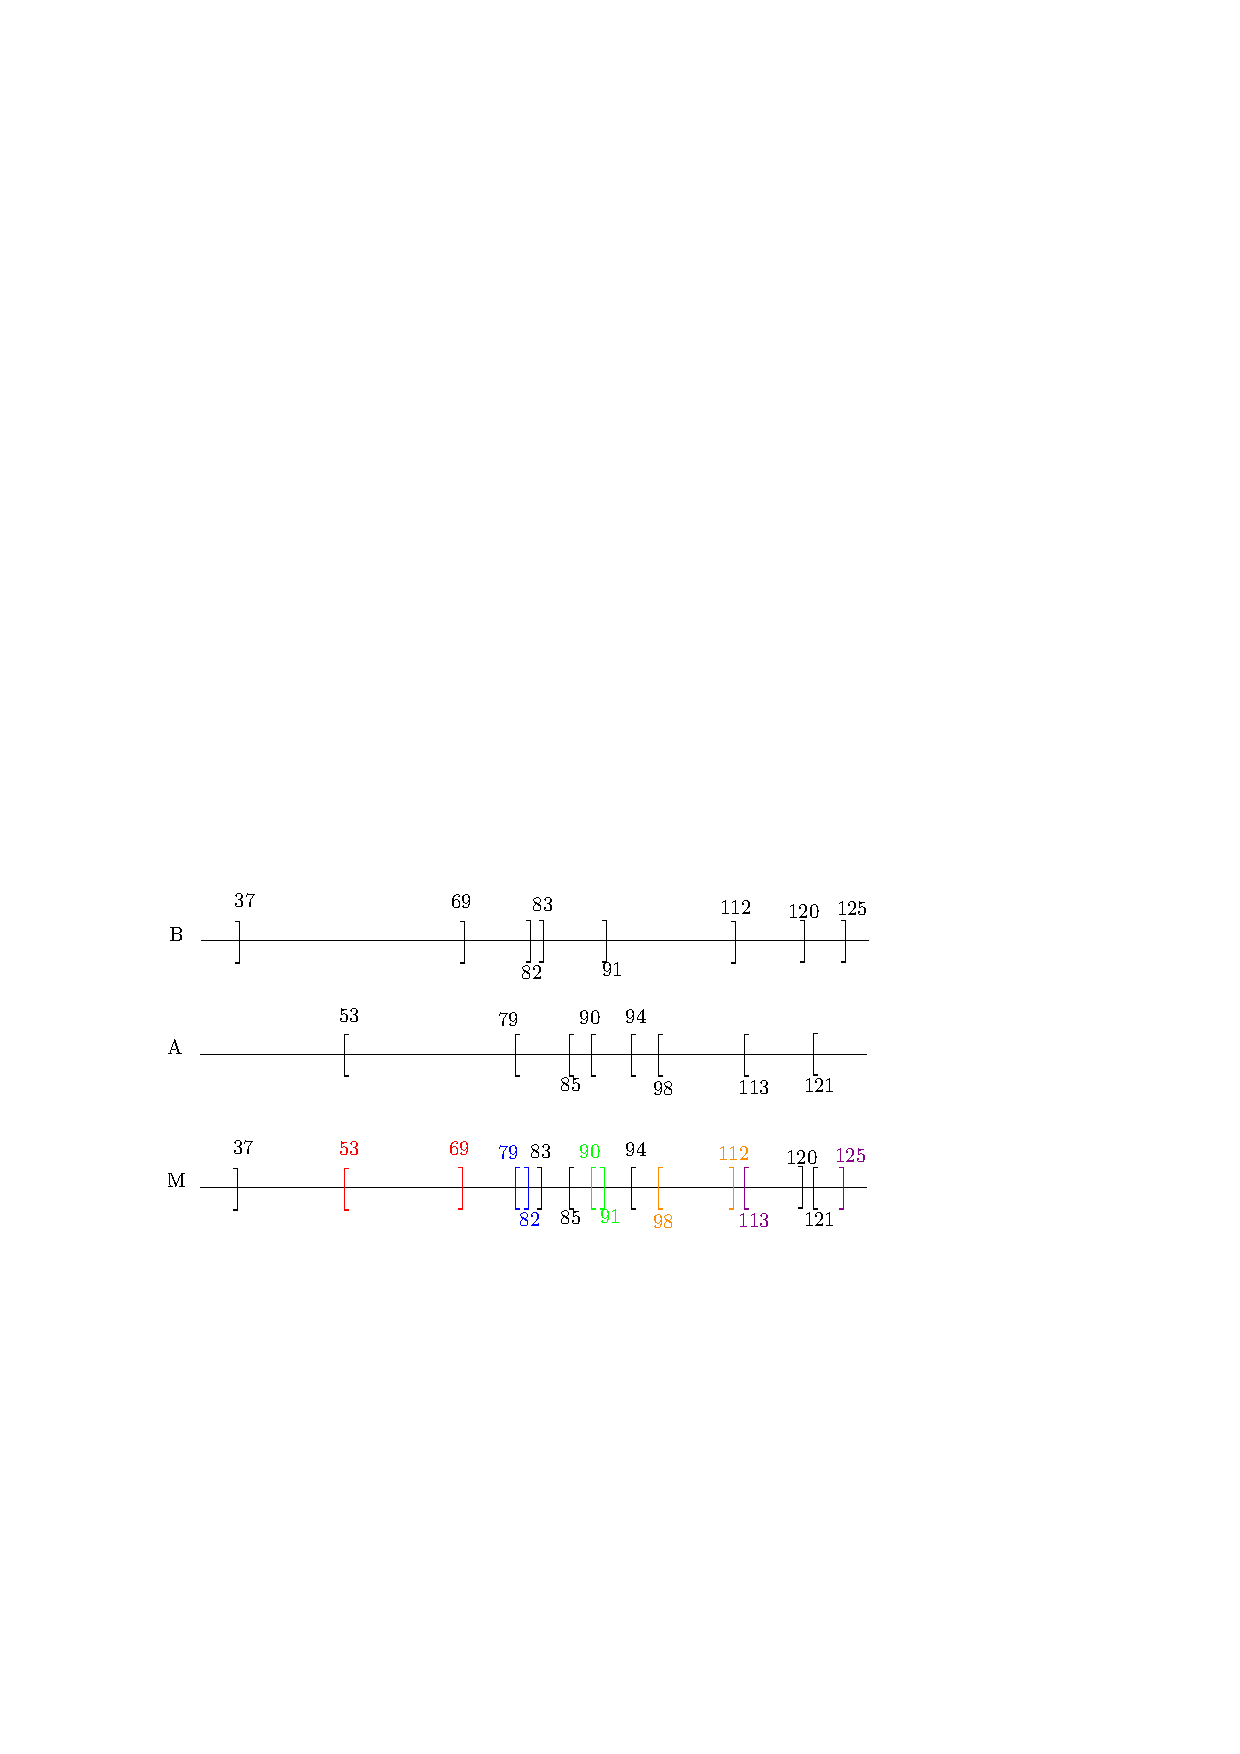
\includegraphics[width=.8\textwidth]{brack_matching.pdf}
\caption{ Bids in $B$ and asks in $A$ are represented using right and left brackets respectively. Every matched bid-ask pair in $M$ is shown using  brackets of same colors. Bids with limit prices $37$, $83$ and $120$ are not matched to any ask in the matching $M$.}
\label{fig:matching}
\end{figure}

More precisely, for a given list of bids $B$ and list of asks $A$, $M$ is a matching iff, (1) All the bid-ask pairs in $M$ are matchable, (2) $B_M$ is duplicate-free, (3) $A_M$ is duplicate-free, (4) $B_M \subseteq B$, and (5) $A_M \subseteq A$.

\begin{definition}
\tw{ \textcolor{gray}{matching\_in} B A M := All\_matchable M $\land$ NoDup $B_M$ $\land$ NoDup $A_M$ $\land$ $B_M \subseteq B$ $\land$ $A_M \subseteq A$.}
\end{definition}
The term \emph{\tw{NoDup $B_M$}} in  the above definition indicates that each bid is a request to trade one unit of item and the items are indivisible.  We use the expression $B_M \subseteq B$  to denote the term \tw{(Subset $B_M$ $B$)}.  It expresses the fact that each element in the list $B_M$ is also present in the list $B$.

\subsection{Lists, sublist and permutation}
While the predicates \tw{NoDup} and  \tw{Subset}  are sufficient to express the notion of a matching, we need more definitions to describe the properties of matching in double sided auctions.  In the following paragraphs we describe three binary relations on lists namely \tw{sublist}, \tw{included} and \tw{perm} which are then used for stating  important results on matching in a double sided auction. 

\begin{figure}[h!]
\centering
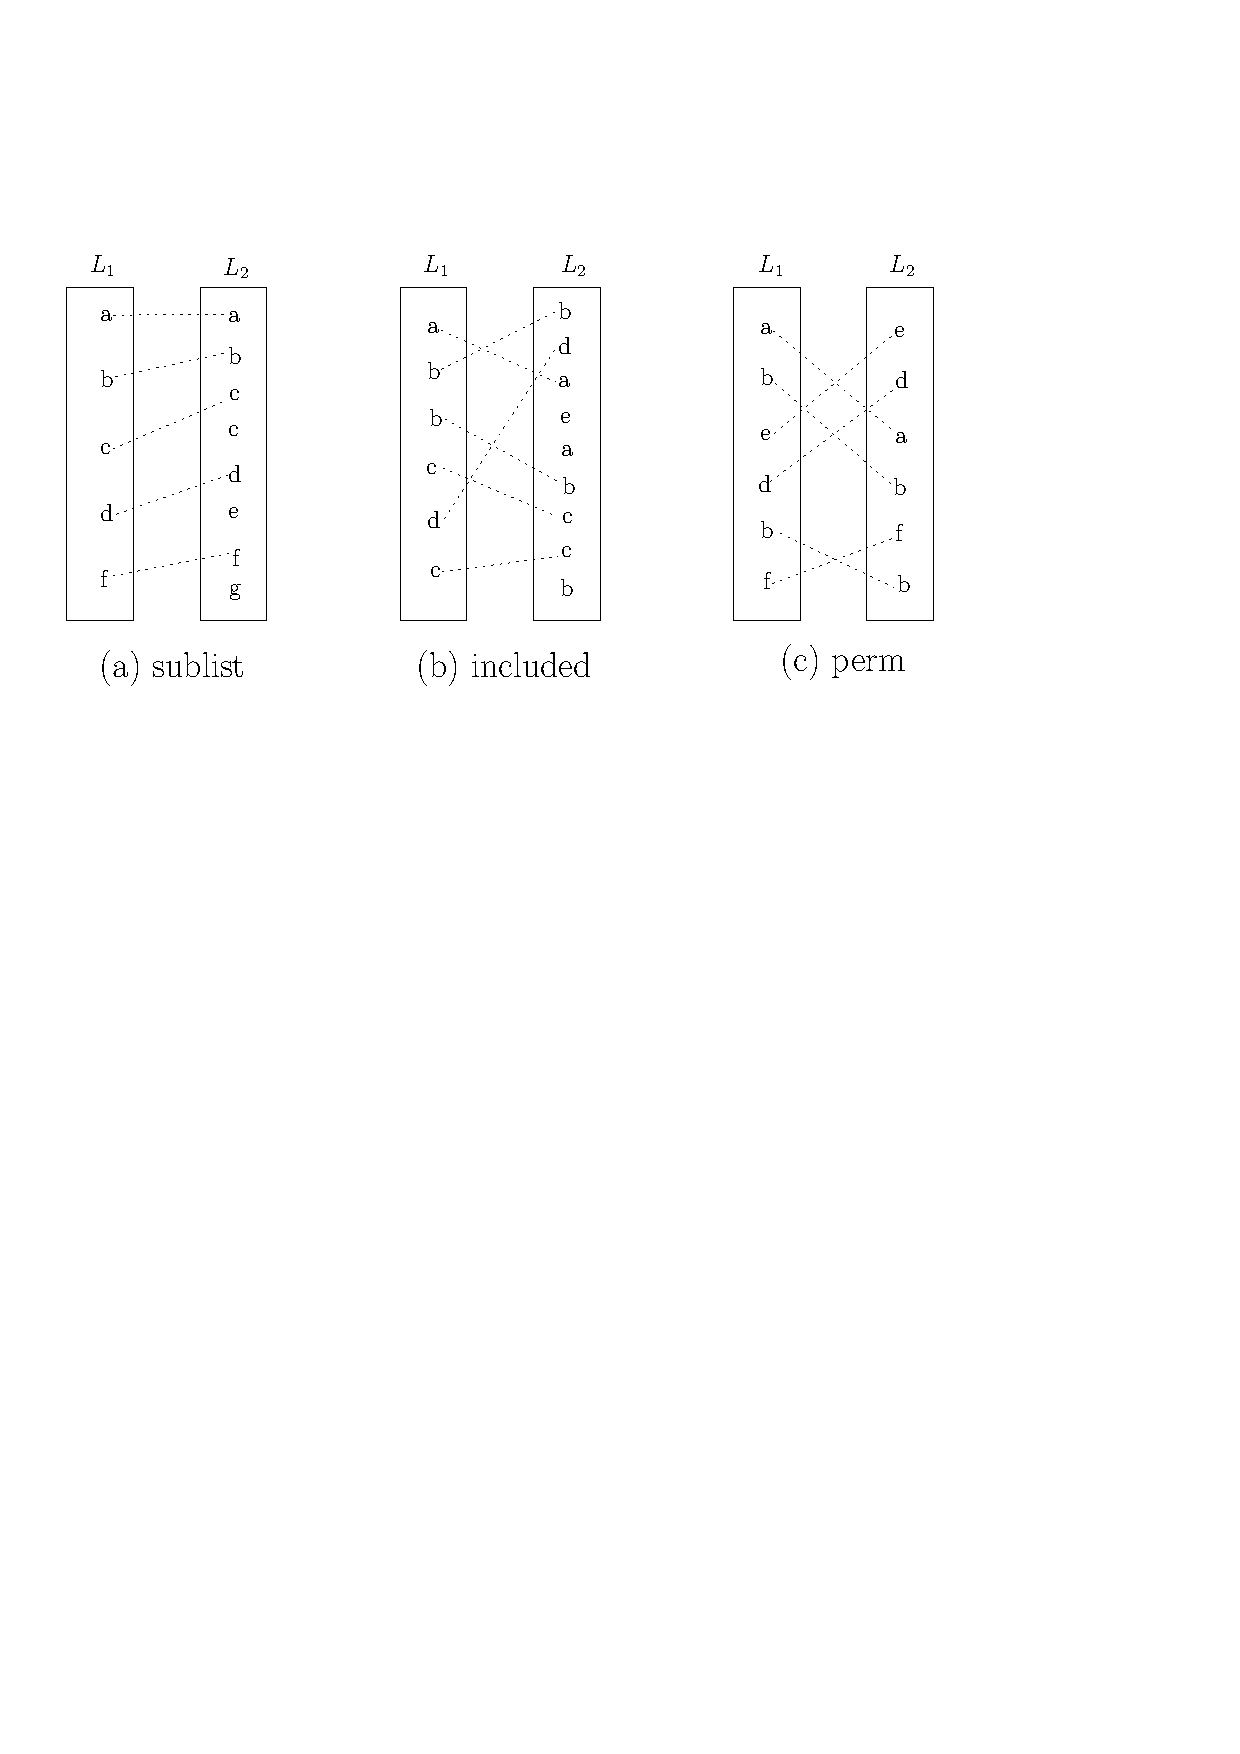
\includegraphics[width=.6\textwidth]{sub_inclu_perm.pdf}
\caption{The dotted lines between the entries of lists confirm the presence of these entries in both the lists. (a) If $L_1$ is \tw{sublist} of $L_2$ then no two dotted lines can intersect. (b) A list $L_1$ is \tw{included} in $L_2$ if every entry in $L_1$ is also present in $L_2$. (c) Two lists $L_1$ and $L_2$ are permutation of each other if each entry has same number of occurrences in both  $L_1$ and $L_2$. }
\label{fig:list}
\end{figure}

\subparagraph*{sublist $L_1$ $L_2$ :} The notion of \tw{sublist}  is analogous to the subsequence relation on sequences. For the given lists $L_1$ and $L_2$ the term  \tw{(sublist $L_1$ $L_2$)} evaluates to \tw{true}  if every entry of $L_1$ is also present in $L_2$ and they appear in the same succession.  For example, in Fig.~\ref{fig:list}(a) the list $L_1$ is a \tw{sublist} of $L_2$ since there is a line incident on each entry of $L_1$ and no two lines intersect each other. 

More precisely,  for any two lists $l$ and $s$ whose elements are of type \tw{T} we have following lemmas specifying the \tw{sublist} relation.

\begin{lemma} 
\tw{ \textcolor{gray}{sublist\_intro1} (a:T): sublist l s-> sublist l (a::s).}
\end{lemma}
\begin{lemma}\label{lem:sublistInd} 
\tw{ \textcolor{gray}{sublist\_elim3a} (a e:T): sublist (a::l)(e::s)-> sublist l s.}
\end{lemma}
\begin{lemma}\label{lem:subCount} 
\tw{ \textcolor{gray}{sublist\_elim4}: sublist l s -> ($\forall$ a, count a l $\leq$ count a s).}
\end{lemma}

The term (\emph{\tw{count a l}}) in Lemma~\ref{lem:subCount}  represents the number of occurrences of element $a$ in the list $l$. Note the recursive nature of \tw{sublist} as evident in Lemma~\ref{lem:sublistInd}. It  makes inductive reasoning easier for the statements which contain \tw{sublist} in the antecedent. However, this is  not true for the other relations (i.e. \tw{included} and \tw{perm}).

\subparagraph*{included $L_1$ $L_2$ :} A list $L_1$ is \tw{included} in  list $L_2$ if every entry of $L_1$ is also present in $L_2$. The notion of \tw{included}  is analogous to the subset relation on multisets. In Fig~\ref{fig:list}(b) the list $L_1$ is \tw{included} in $L_2$ since there is a line incident on each entry of $L_1$. More precisely, we have following lemmas specifying the \tw{included} relation.
\begin{lemma}
\tw{\textcolor{gray}{included\_intro}: ($\forall$ a, count a l $\leq$ count a s)-> included l s.}
\end{lemma}
\begin{lemma}
\tw{ \textcolor{gray}{included\_elim}: included l s -> ($\forall$ a, count a l $\leq$ count a s).}
\end{lemma}
\begin{lemma}
\tw{ \textcolor{gray}{included\_intro3}: sublist l s -> included l s. }
\end{lemma}

Note that if $l$ is \tw{sublist} of $s$ then $l$ is also \tw{included} in $s$ but not the vice versa. However, if both the lists $l$ and $s$ are sorted based on some ordering on type \tw{T} then $l$ is \tw{sublist} of $s$ whenever $l$ is \tw{included} in $s$.
\begin{lemma}
\tw{ \textcolor{gray}{sorted\_included\_sublist}: Sorted l -> Sorted s -> included l s -> sublist l s.}
\end{lemma}

\subparagraph*{perm $L_1$ $L_2$ :} A list $L_1$  is permutation of list $L_2$  iff $L_1$  is included in $L_2$ and $L_2$ is included in $L_1$.  The notion of permutation for lists is similar to the equality in multisets. In Fig~\ref{fig:list}(c) the list $L_1$  is perm of list $L_2$. We have the following lemmas specifying the essential properties of the \tw{perm} relation.

\begin{lemma}
\tw{ \textcolor{gray}{ perm\_intro}: ($\forall$ a, count a l = count a s) -> perm l s.}
\end{lemma}
\begin{lemma}
\tw{ \textcolor{gray}{perm\_elim}: perm l s -> ($\forall$ a, count a l = count a s).}
\end{lemma}
\begin{lemma}\label{lem:permSort}
\tw{ \textcolor{gray}{perm\_sort}(e: T-> T-> bool): perm l s -> perm  l (sort e s).}
\end{lemma}

The term (\emph{\tw{sort s}}) in Lemma~\ref{lem:permSort} represents the list $s$ sorted using an ordering relation \tw{e}. The definition of matching as a list is necessary for describing processes that operate on it. However, while describing various properties of a matching we can always consider it as a collection. For example, consider the following lemma which states that the property of  being a matching is invariant over permutation. 
\begin{lemma}
\tw{\textcolor{gray}{match\_inv}: perm M  M' -> perm B B' -> perm A A' -> matching\_in B A M -> matching\_in B' A' M'. }
\end{lemma}
We use $B_M$ to represent the list of bids from $B$ that are matched in  $M$. Similarly we  use notation $P_M$ to represent  a list containing trade prices of matched bid-ask pair in $M$. While proving various properties of a matching $M$ we very often base our arguments solely on the information present in $B_M$, $A_M$ and $P_M$. Therefore it is useful to have lemmas establishing the interaction of  $B_M$, $A_M$ and $P_M$ with above mentioned relations on lists. 

\begin{lemma}
\tw{\textcolor{gray}{included\_M\_imp\_included\_bids}:included $M$  $M'$ -> included $B_M$ $B_{M'}$ }.
\end{lemma}

\begin{lemma}
\tw{\textcolor{gray}{included\_M\_imp\_included\_asks}:included $M$  $M'$ -> included $A_M$ $A_{M'}$ }
\end{lemma}

\begin{lemma}
\tw{\textcolor{gray}{included\_M\_imp\_included\_tps}:included $M$  $M'$ -> included $P_M$ $P_{M'}$  }
\end{lemma}

\begin{lemma}
\tw{\textcolor{gray}{sorted\_nodup\_is\_sublistB}: Sorted $B$ -> Sorted  $B'$ -> NoDup $B$ -> NoDup $B'$ ->  $ B \subseteq B'$  -> sublist $P_B$ $P_B'$. }
\end{lemma}

\section{Analysis of Double sided auctions}\label{sec:analysis}
Usually in a double sided auction mechanism, the profit of an auctioneer is the difference between the limit prices of matched bid-ask pair. In this work we do not consider analysis of profit for the auctioneer. Therefore the buyer of a matched bid-ask pair pays the same amount which the seller receives. This price for a matched  bid-ask pair is called the trade price for that pair. Since the limit price for a buyer is the price above which she doesn't want to buy, the trade price for this buyer is expected to be below its limit price. Similarly the limit price for a seller is the price below which he doesn't want to sell, hence the trade price for this seller is expected to be below its limit price. Therefore in any matching it is desired that the trade price of a bid-ask pair lies between their limit prices. A matching which has this property is called an \emph{individual rational (IR)} matching. Note that any matching can be converted to an IR matching without altering its bid-ask pair (See Fig~\ref{fig:IR}).

\begin{figure}[h!]
\centering
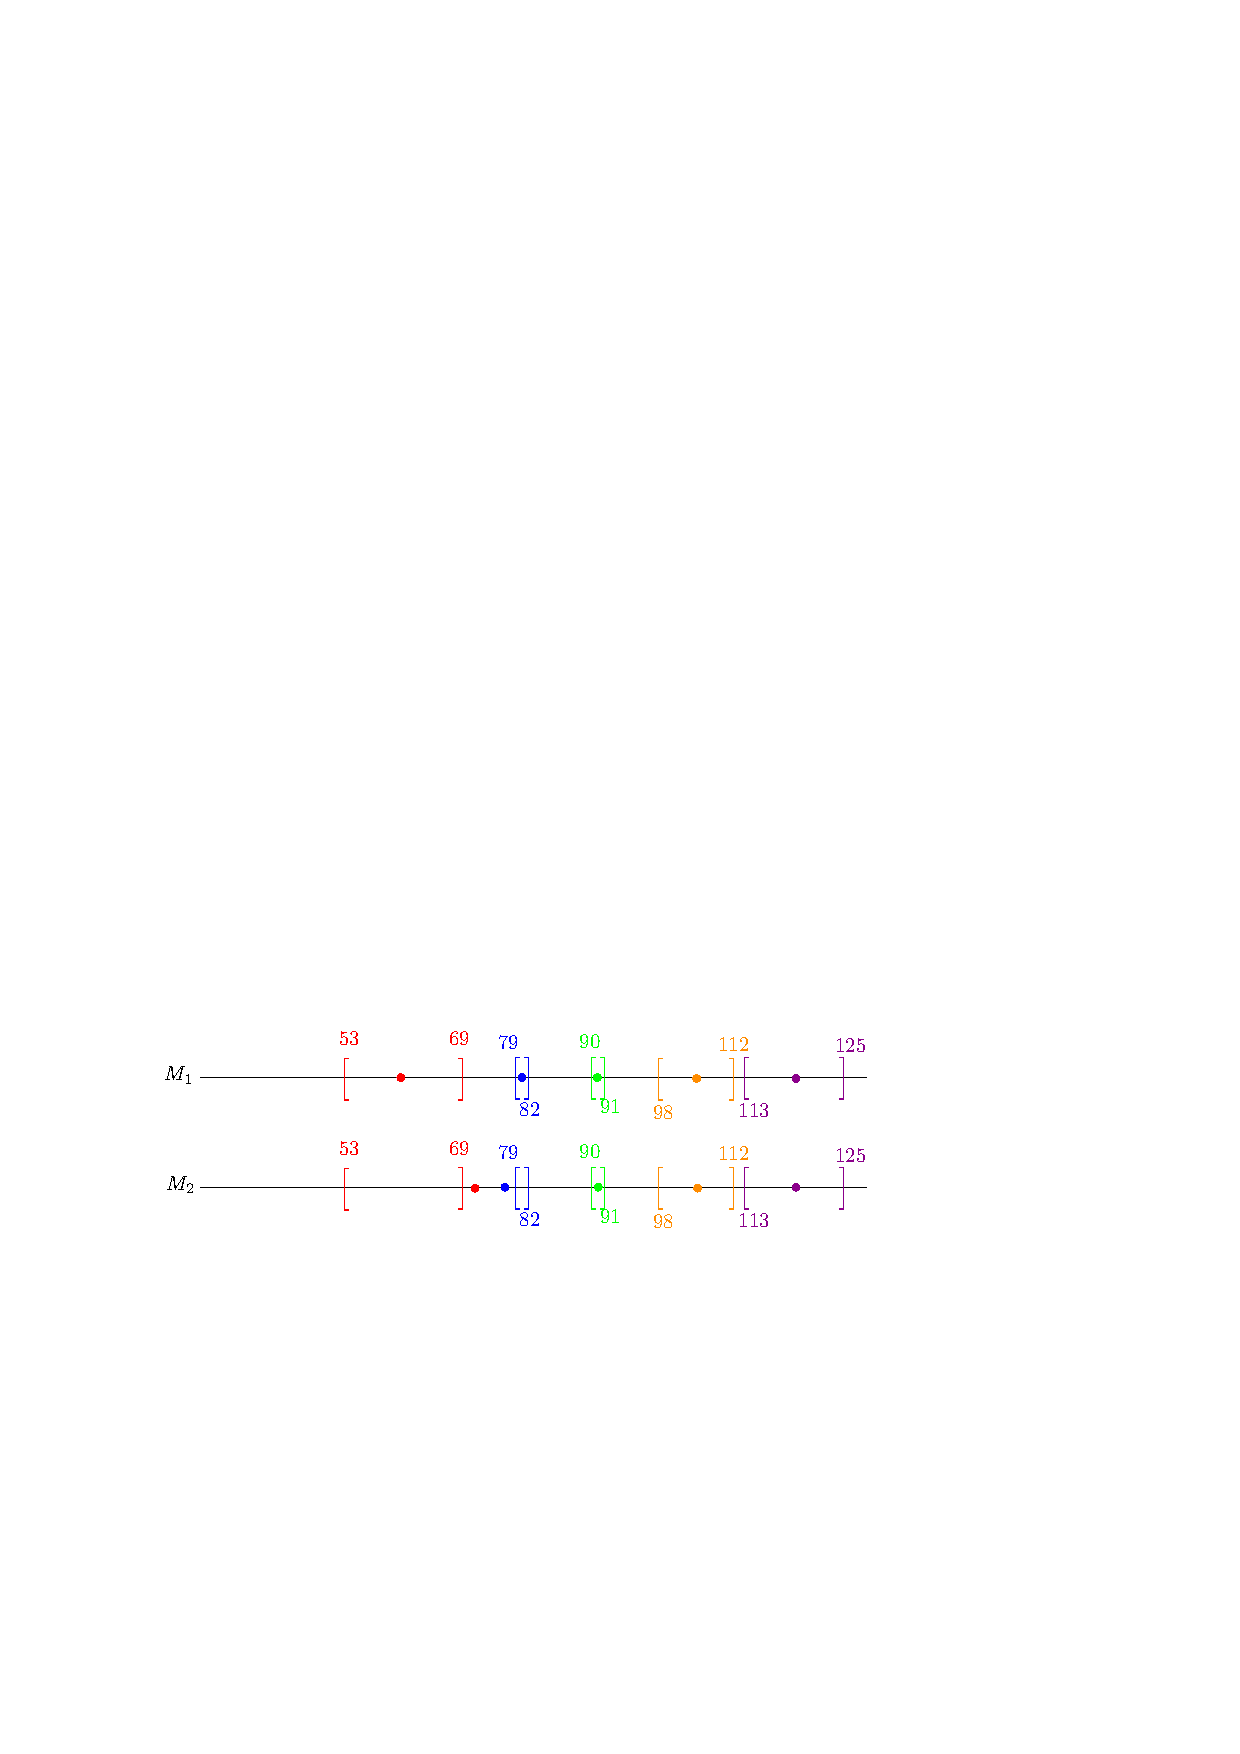
\includegraphics[width=.8\textwidth]{brack_IR.pdf}
\caption{ The colored dots represent the trade prices at which the corresponding matched bid-ask pairs are traded. While the matching $M_2$ is not IR since some dots lie outside the corresponding matched bid ask-pair. The matching $M_1$ is IR because trade prices for every matched bid-ask pair  lie inside the interval. Note that the matching $M_1$ and $M_2$ contains exactly the same bid-ask pairs.}
\label{fig:IR}
\end{figure}

The number of matched bid-ask pairs produced by a matching algorithm is crucial in the design of a double sided auction mechanism. Increasing the number of matched bid-ask pairs increases  liquidity in the market. Therefore, producing a maximum matching is an important aspect of double sided auction mechanism design. For a given list of bids $B$ and list of asks $A$ we say a matching $M$ is  a maximum matching if no other matching $M'$ on the same $B$ and $A$ contains more matched bid-ask pairs than $M$. 

\begin{definition}
\tw{ \textcolor{gray}{Is\_MM} M B A := (matching\_in B A M) $\land$ 
($\forall$ M', matching\_in B A M' $\rightarrow$ |M'| $\leq$ |M|)}.
\end{definition}

In certain situations, to produce a maximum matching, different bid-ask pairs must be assigned different trade prices. For example see Fig ~\ref{fig:mmum}. To get a maximum matching of size two it is necessary to trade both the matched bid-ask pairs at different prices.  However, different prices for the same product in the same market simultaneously leads to dissatisfaction amongst some of the traders. A mechanism which clears all the matched bid-ask pairs at same trade price is called a \emph{uniform matching}. It is also known as \emph{perceived-fairness}. 

\begin{figure}[h!]
\centering
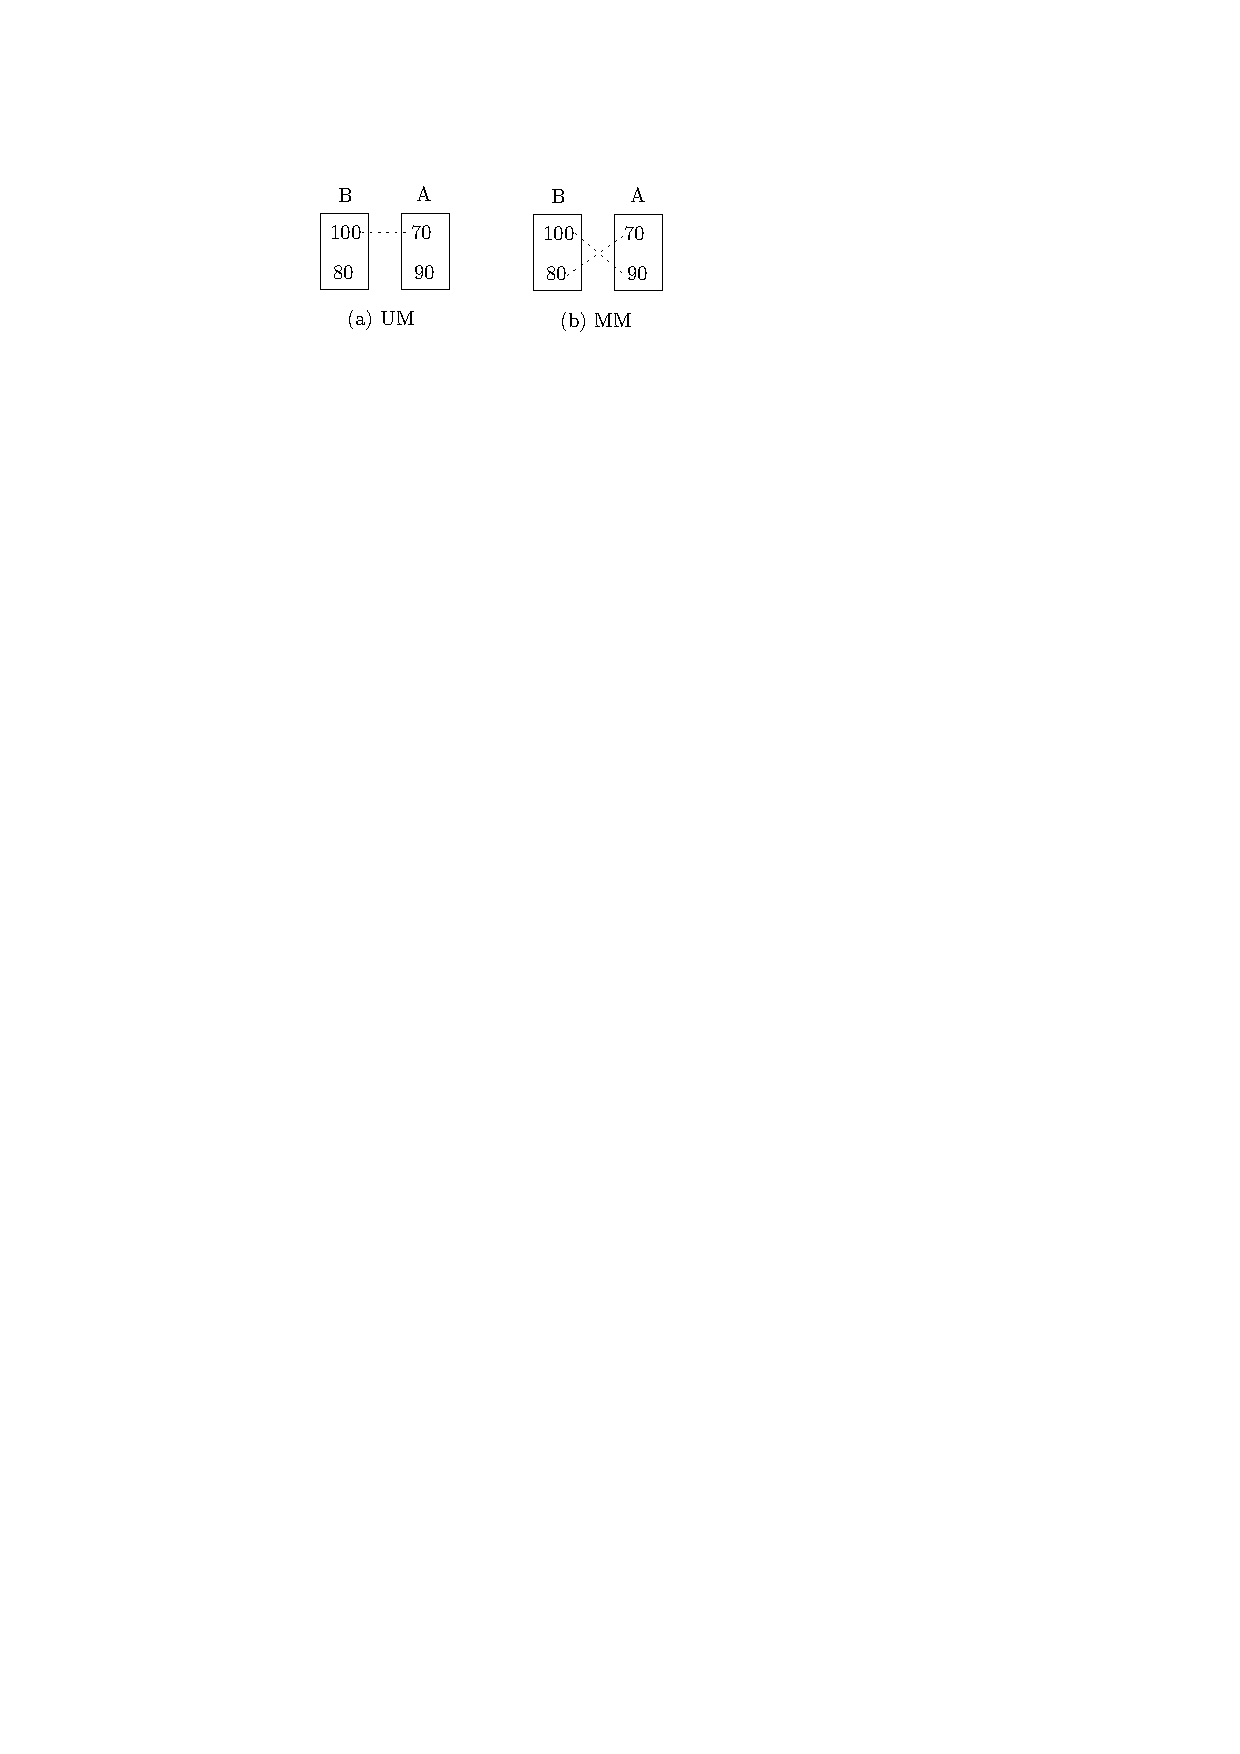
\includegraphics[width=.5\textwidth]{mm_um.pdf}
\caption{In this figure two bids with limit prices 100 and 80 respectively are matched against two asks of limit price 70 and 90. There is only one matching $M_2$ of size two possible and it is not uniform.}
\label{fig:mmum}
\end{figure}

\subsection{Fairness}  

A bid with higher limit price is more competitive compared to bids with lower limit prices. Similarly an ask with lower limit price is more competitive compared to asks with higher limit prices. In a competitive market, like double sided auction, it is necessary to prioritise more competitive traders for matching. A matching which prioritises more competitive traders is called a \emph{fair} matching. Consider the following predicates \tw{fair\_on\_bids} and  \tw{fair\_on\_asks} which are used to describe a fair matching. 

\begin{definition}
\tw{ \textcolor{gray}{fair\_on\_bids} M B:=
$\forall$ b b', In b B $\land$ In b' B -> b $>$ b' -> In b' $B_M$ -> In b $B_M$.}
 \end{definition}
\begin{definition}
\tw{ \textcolor{gray}{fair\_on\_asks} M A:=
$\forall$ s s', In s A $\land$ In s' A -> s $<$ s' -> In s' $A_M$ -> In s $A_M$. }
\end{definition}
\begin{definition}
\tw{ \textcolor{gray}{Is\_fair} M B A:=
fair\_on\_asks M A $\land$ fair\_on\_bids M B.}
\end{definition}

Here, the predicate \tw{fair\_on\_bids M B}  states that the matching $M$  is fair for the list of buyers $B$. Similarly,  the predicate \tw{fair\_on\_asks M A} states that the matching $M$  is fair for the list of sellers $A$.  A matching which is fair on both the traders (i.e. $B$ and $A$) is expressed using the predicate \tw{Is\_fair M B A}.

Unlike the uniform matching, a fair matching can always be achieved without compromising the size of matching. We can accomplish this by converting any matching into a fair matching without changing its size. For example, consider the following function \tw{make\_FOB}.

\begin{verbatim}
	  Fixpoint Make_FOB (M:list fill_type) (B: list Bid):=
	    match (M,B) with 
	    |(nil,_) => nil
	    |(m::M',nil) => nil
	    |(m::M',b::B') => (Mk_fill b (ask_of m) (tp m))::(Make_FOB M' B')
	  end.
\end{verbatim}

The function \tw{make\_FOB} produces a \tw{fair\_on\_bids} matching from a given matching M and a list of bids B, both sorted in decreasing order of bid prices (See Fig~\ref{fig:fair}). The function \tw{make\_FOB} is a recursive function and  at each step it replaces the largest bid in M with the largest bid available in B. Since at any moment the largest bid in B is bigger than the largest bid in M, the new bid-ask pair is still matchable. Note that \tw{make\_FOB} doesn't change any of the ask in M and due to the recursive nature of \tw{make\_FOB} on B, a bid is not repeated in the process of replacement.  This ensures that the new $B_M$ is duplicate-free. Once a matching is modified to a fair matching on bids, we use similar function \tw{make\_FOA} on this matching to produce a fair on ask matching. Hence the final result is a fair matching. 

\begin{figure}[h!]
\centering
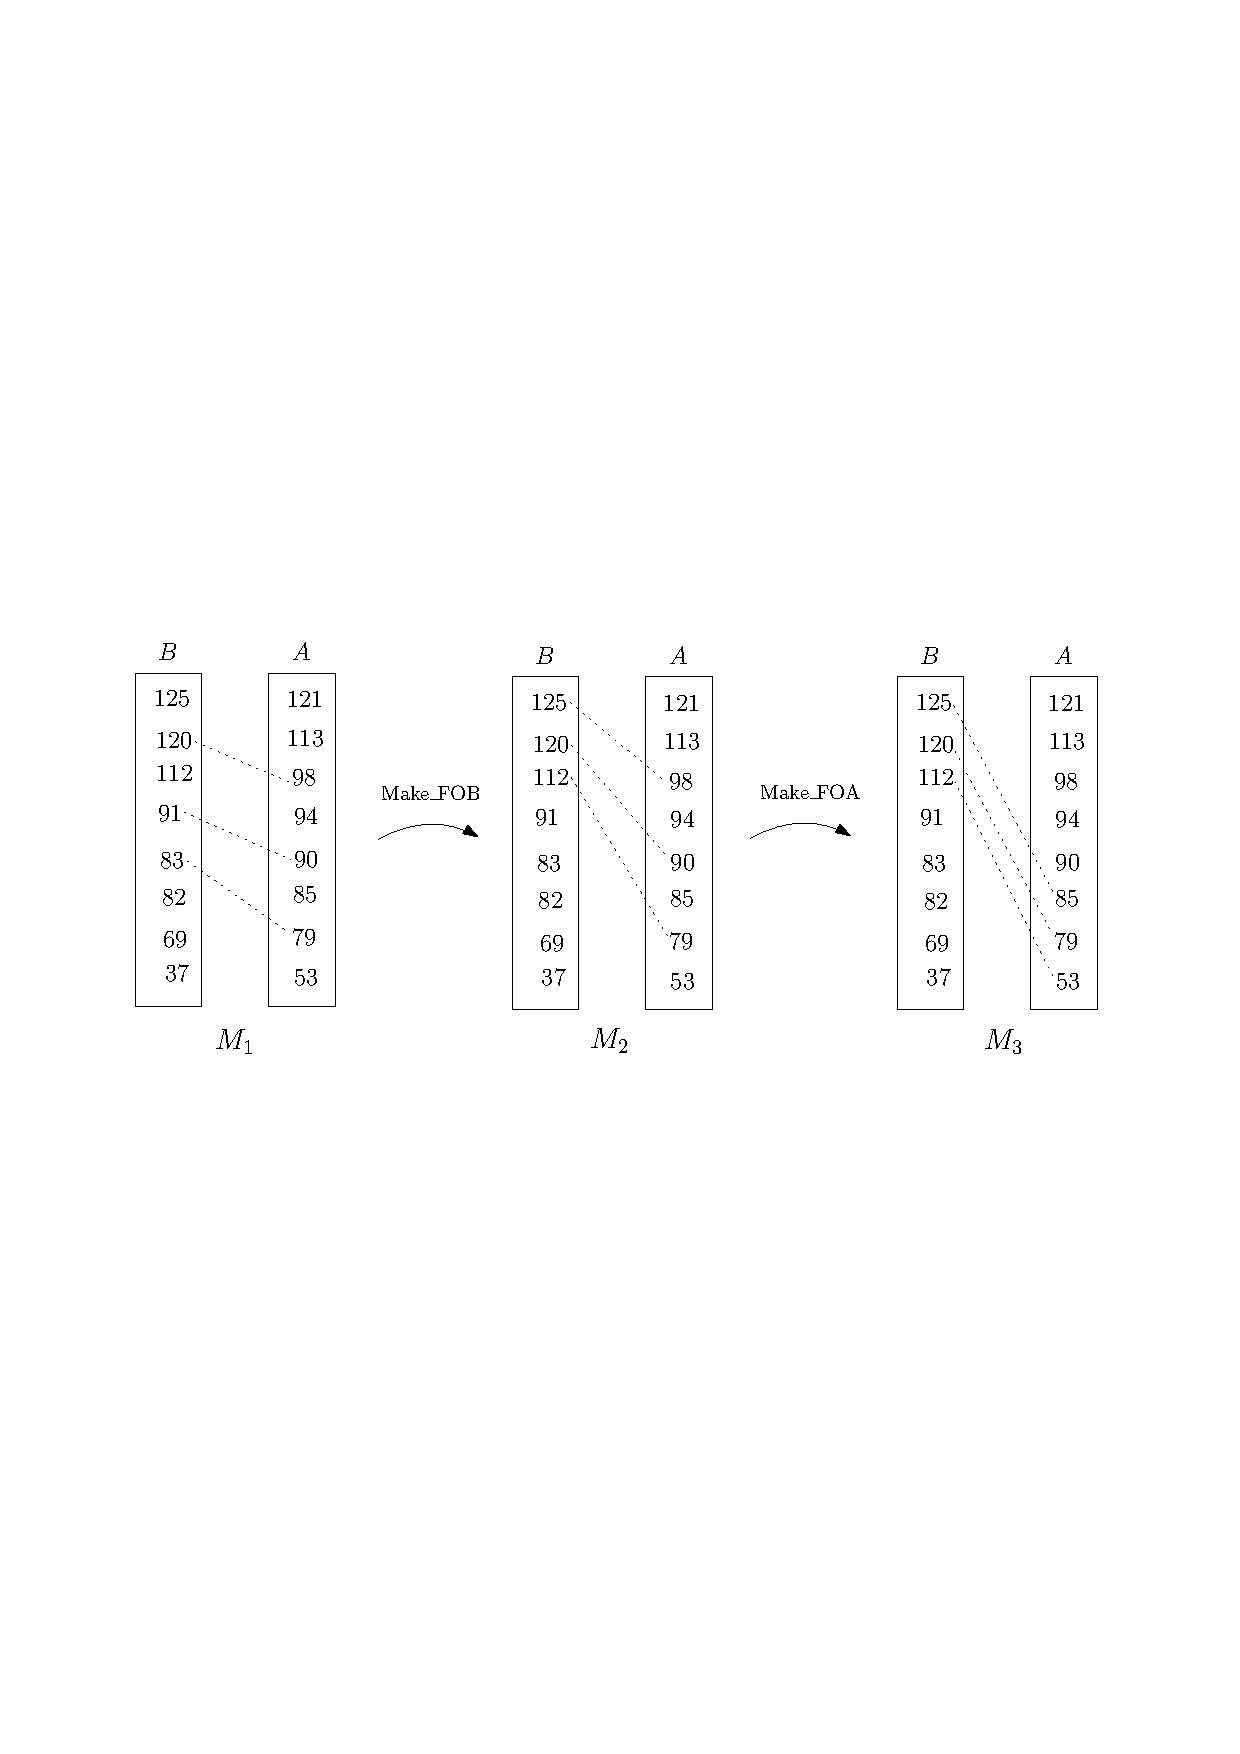
\includegraphics[width=.8\textwidth]{make_fair.pdf}
\caption{The dotted lines in this figure represent  matched bid-ask pairs in  matching $M_1$, $M_2$ and $M_3$. In the first step function \tw{make\_FOB} operates on $M_1$ recursively. At each step it picks the top bid-ask pair, say $(b,a)$ in $M_1$ and replaces the bid  $b$ with a most competitive bid available in $B$. The result of this process is a \tw{fair\_on\_bids} matching $M_2$. In a similar way the function \tw{make\_FOA} changes $M_2$ intro a fair on ask matching $M_3$.  }
\label{fig:fair}
\end{figure}

More precisely, for the function \tw{make\_FOB} and \tw{make\_FOA} we have the following lemmas proving it fair on bids and fair on asks respectively. 
\begin{lemma}\label{lem:fob}
\tw{ \textcolor{gray}{mfob\_fair\_on\_bid} M B:
  (Sorted M) -> (Sorted B) -> sublist $P_{B_M}$ $P_B$ ->
  fair\_on\_bids (Make\_FOB M B) B.  }
\end{lemma}

\begin{lemma}\label{lem:foa}
\tw{ \textcolor{gray}{mfob\_fair\_on\_ask} M A: 
 (Sorted M) -> (Sorted A) -> sublist $P_{A_M}$ $P_A$ ->
  fair\_on\_asks (Make\_FOA M A) A.  }
\end{lemma}

\begin{theorem}\label{thm:fairMatching}
\tw{ \textcolor{gray}{exists\_fair\_matching} (Nb: NoDup B)(Na: NoDup A): 
 matching\_in B A M -> ( $\exists$ M', matching\_in B A M' $\land$ Is\_fair M' B A $\land$ |M| = |M'|). }
\end{theorem}

Proof of Theorem~\ref{thm:fairMatching} depends on Lemma \ref{lem:foa} and Lemma \ref{lem:fob}. Furthermore, Lemma \ref{lem:foa} and Lemma \ref{lem:fob} can be proved using induction on the size of M. 

\subsection{Maximum Matching}

The liquidity in any market is a measure of how quickly one can trade in the market without much cost. A highly liquid market boosts the investor's confidence in the market. One way to increase the liquidity in a double sided auction is to maximize the number of matched bid-ask pairs. In the previous section we have seen that any matching can be changed to a fair matching without altering its size. Therefore, we can have a maximum matching without compromising on the fairness of the matching. In this section we describe a matching which is fair as well as maximal. For a given list of bid $B$ and list of ask $A$, a maximum and fair matching can be achieved in two steps. In the first step we apply function \tw{produce\_MM} which produces a matching which is maximal and fair on bids. In the next step we apply \tw{make\_FOA} to this maximum matching to produce a fair on ask matching (See Fig~\ref{fig:mm}).

\begin{figure}[h!]
\centering
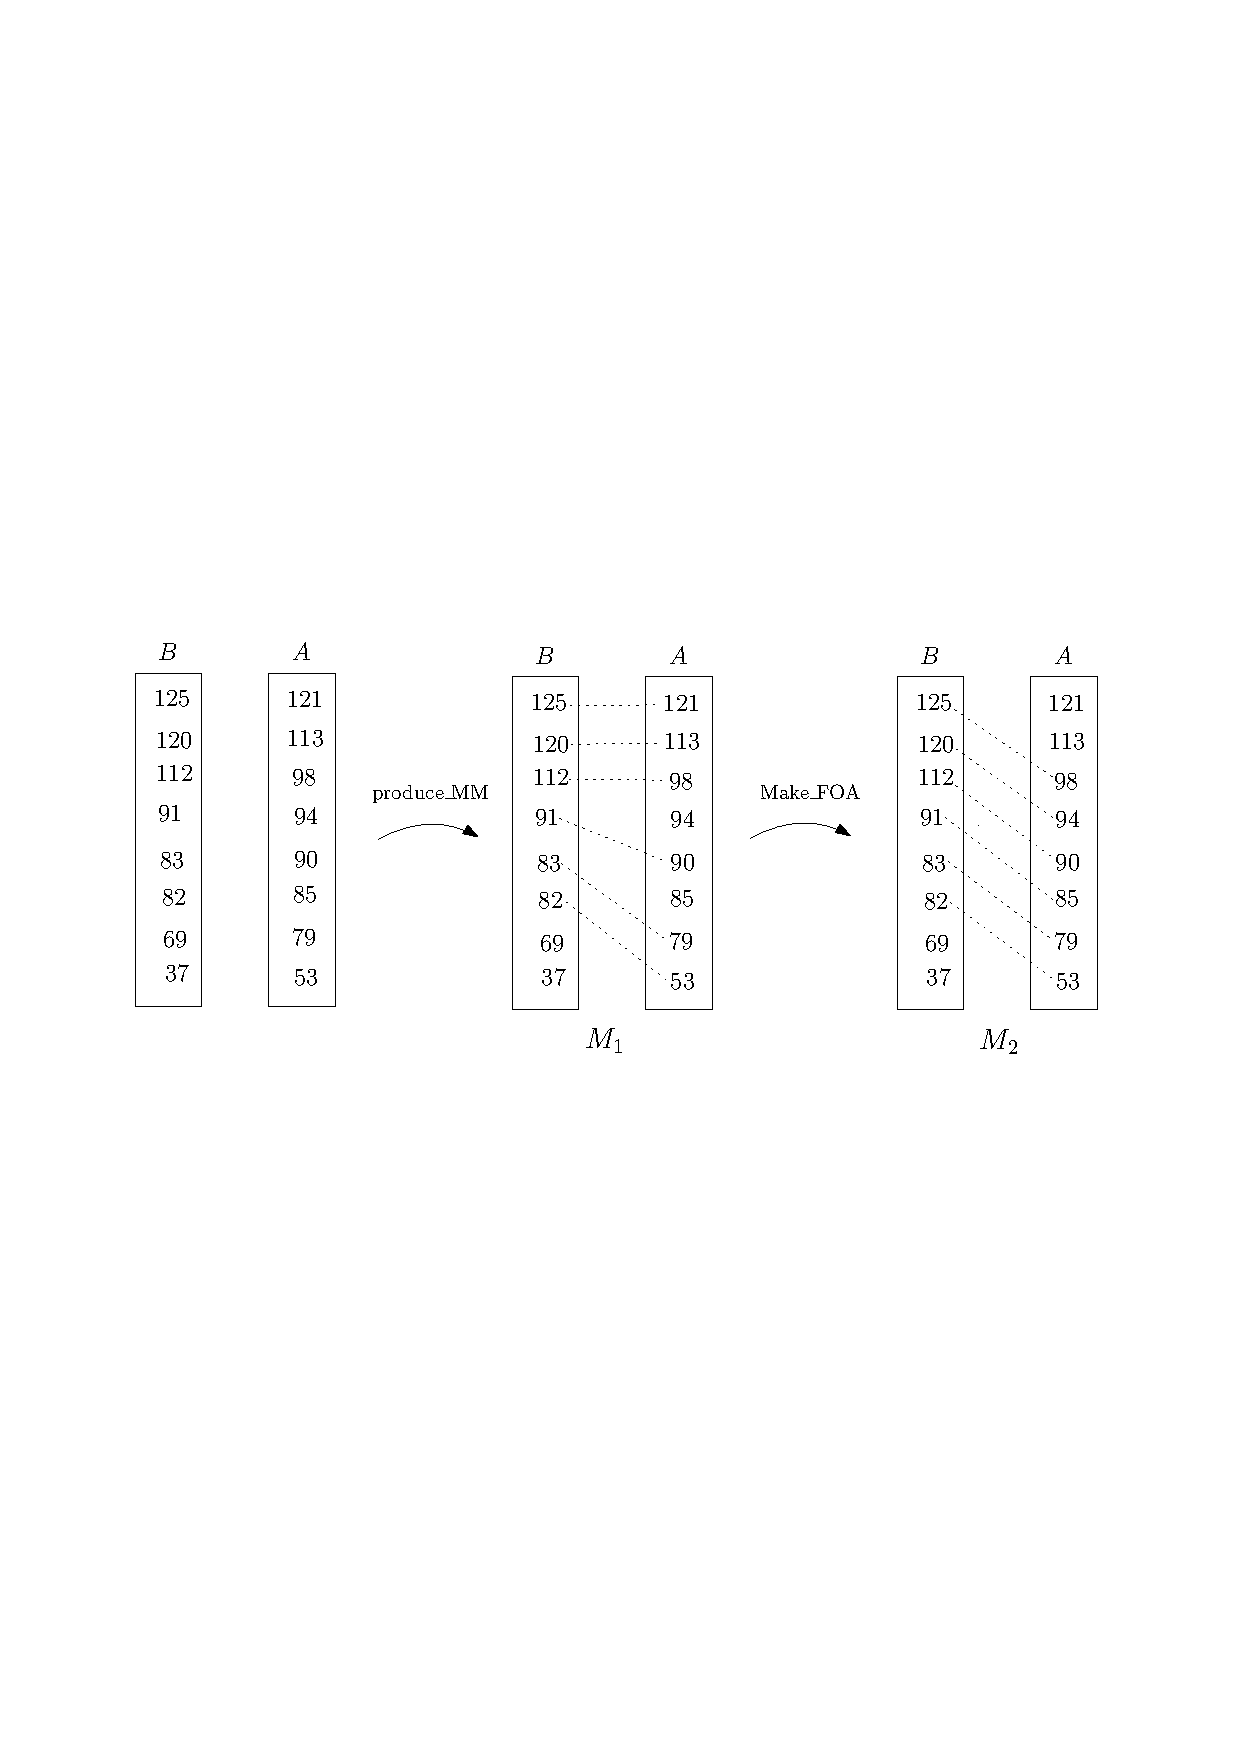
\includegraphics[width=.8\textwidth]{MM.pdf}
\caption{In the first step, the function \tw{produce\_MM} operates recursively on the list of bids B and list of asks A. At each step the function \tw{produce\_MM} selects a most competitive available bid and then pairs it with the largest matchable ask. Note that the output of this function is fair on bids since it doesn't leave any bid from top. In the second step, the function \tw{make\_FOA} converts  $M_1$ into fair matching $M_2$. }
\label{fig:mm}
\end{figure}

\begin{verbatim}
Fixpoint produce_MM (B:list Bid) (A: list Ask): (list fill_type) :=
  match (B, A) with
  |(nil, _) => nil
  |(b::B', nil) => nil              
  |(b::B', a::A') =>  match (a <= b) with
     |true => ({|bid_of:= b; ask_of:= a; tp:=(bp b)|})::(produce_MM B' A')
     |false => produce_MM B A'
    end
  end. 
\end{verbatim}

At each iteration the above function generates a matchable bid-ask pair (See Fig~\ref{fig:mm}). Due to the recursive nature of  function  \tw{produce\_MM} on both $B$ and $A$, it never pairs any bid with more than one asks. This ensures that the list of bids in matching (i.e. $B_M$) is duplicate-free. Note that the function \tw{produce\_MM} tries to match a bid until it finds a matchable ask. The function terminates when either all the bids are matched or it encounters a bid for which no matchable ask is available.  Therefore, the function \tw{produce\_MM} produces a matching from a given lists of bids $B$ and a list of asks $A$, both sorted in decreasing order by there limit prices.  

The following theorem states that when the function \tw{produce\_MM} is given a list of bids $B$ and list of asks $A$, both sorted in decreasing order by limit prices, then it produces a maximum matching.
\begin{theorem}
\tw{\textcolor{gray}{produce\_MM\_is\_MM}(Nb:NoDup B)(Na:NoDup A): Sorted  B -> Sorted A -> Is\_MM (produce\_MM B A) B A. }
\end{theorem}
\textbf{Proof}: We prove this result using induction on the size of list $A$. 
\begin{itemize}
\item Induction hypothesis (\tw{IH}): \emph{ \tw{ $\forall$ A', |A'| < |A| -> $\forall$ B, Sorted  B -> Sorted A' -> Is\_MM (produce\_MM B A') B A'.} }
\end{itemize}
Let $M$ be an arbitrary matching on the list of bids $B$ and list of asks $A$. Moreover, assume that $b$ and $a$ are the topmost bid and ask present in $B$ and $A$ respectively (i.e. $A = (a::A')$ and $B = (b::B')$). We need to prove that $|M| \leq$ |\tw{produce\_MM} $B$ $A$|.  We prove this inequality in  the following two cases.
\begin{itemize}
\item \textbf{Case-1} ($b<a$): In this case the limit price of $a$ is strictly more than the limit price of $b$.  In this case the function \tw{produce\_MM} computes a matching on $B$ and $A'$. Note that due to the induction hypotheses (i.e. \tw{IH}) this is a maximum matching for $B$ and $A'$. Since the limit price of ask $a$ is more than the most competitive bid $b$ in $B$ it cannot be present in any matching of $B$ and $A$. Therefore a maximum matching on $B$ and $A'$ is also a maximum matching on $B$ and $A$. Hence we have |$M$| $\leq$ | \tw{produce\_MM} $B$ $A$ |.
\item \textbf{Case-2} ($a \leq b$): In this case the function \tw{produce\_MM} produces a matching of size $m + 1$ where $m$ is the size of matching \tw{produce\_MM $B'$ $A'$}.  Hence we need to prove that \tw{$|M|$ $\leq$ $m+1$}. Note that due to induction hypothesis (i.e. \tw{IH}) the matching \tw{produce\_MM $B'$ $A'$} is a maximum matching on $B'$ and $A'$.  Hence no matching on $B'$ and $A'$ can have size bigger than $m$. Without loss of generality we can assume that $M$ is also sorted in decreasing order of bid prices. Now we further split this case into the following five sub cases (see Fig~\ref{fig:mmProof}).

\begin{figure}[h!]
\centering
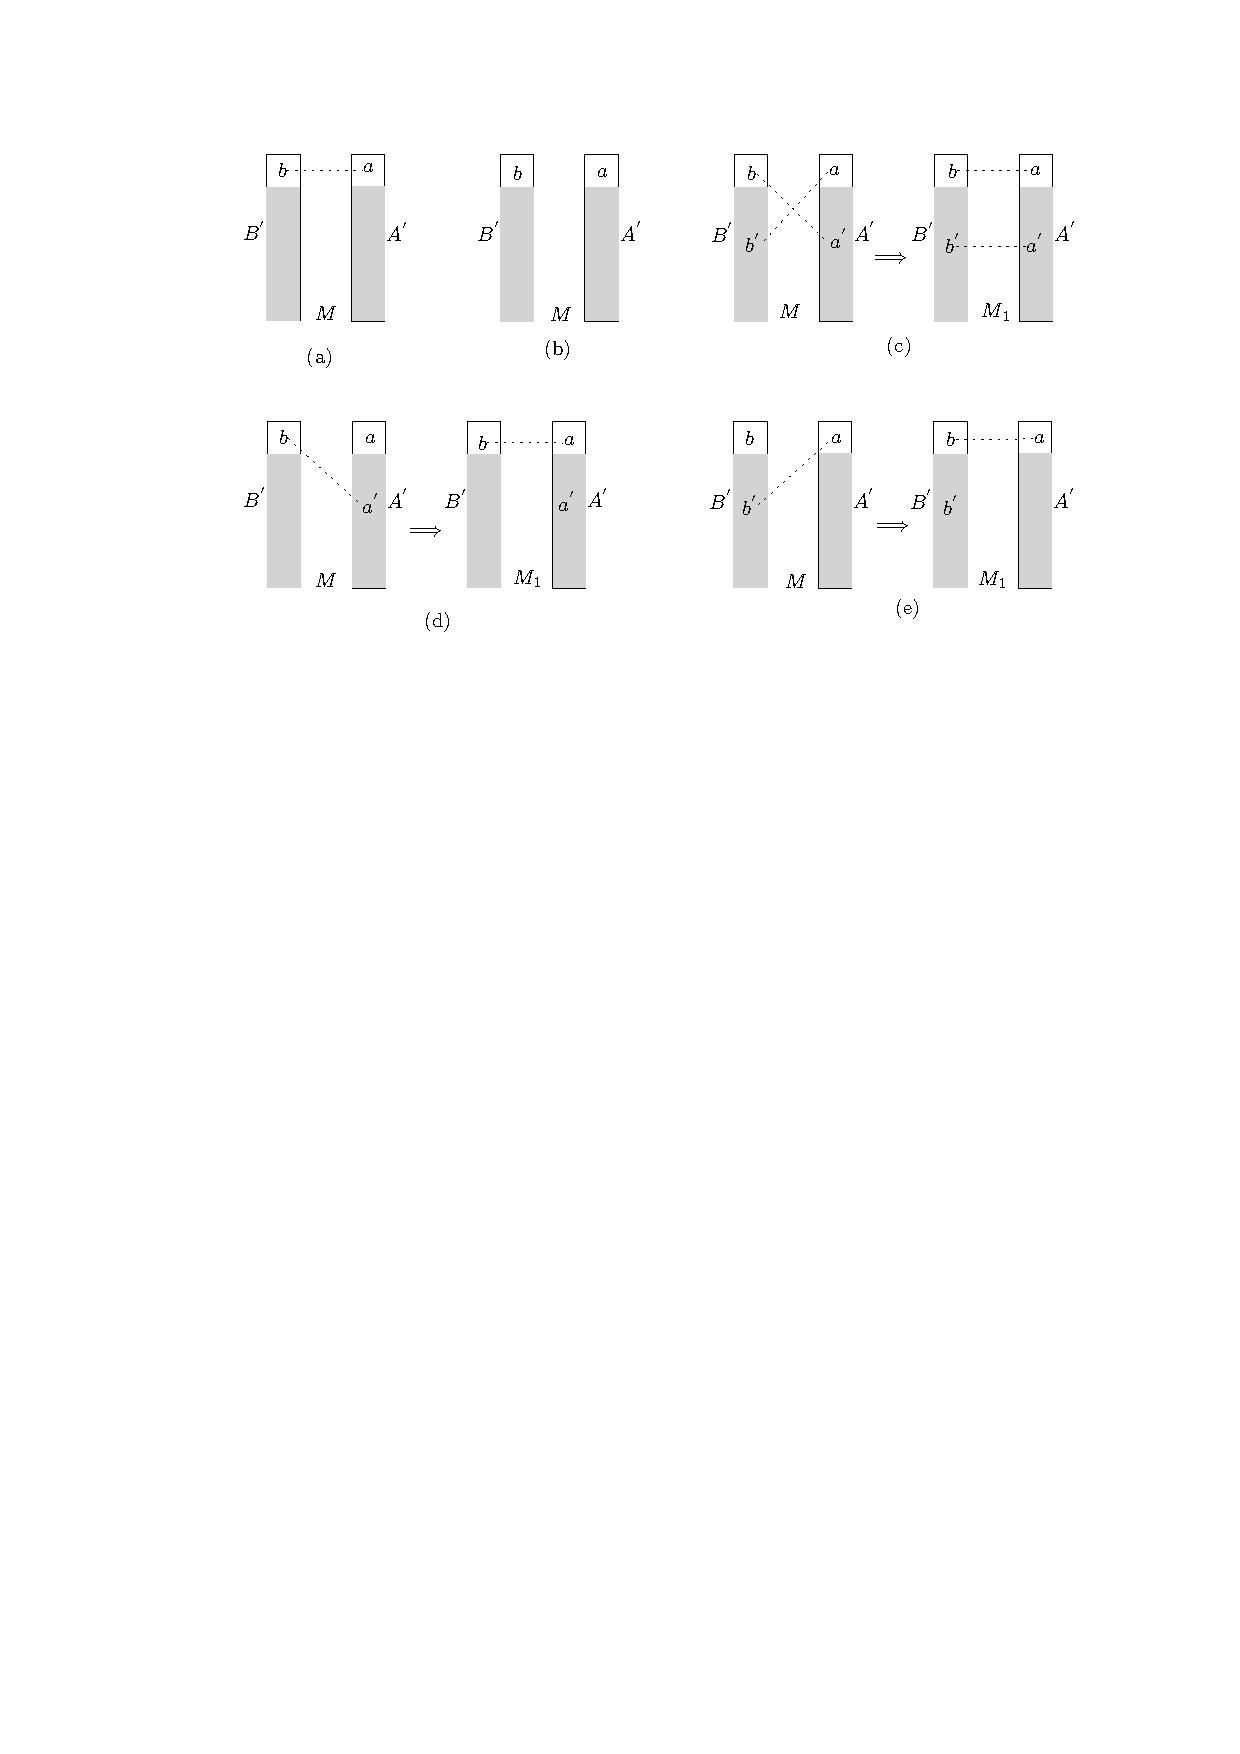
\includegraphics[width=1\textwidth]{mm_proof.pdf}
\caption{This figure shows all the five sub cases of Case-2 (i.e. when $b \geq a$). The dotted line shows presence of the connected pair in matching $M$.  Both the list of bids $B$ and list of asks $A$ are sorted in decreasing order of their limit prices. Moreover, we assume $B = b::B'$ and $A = a::A'$.  }
\label{fig:mmProof}
\end{figure}

\begin{itemize}
\item \textbf{Case-2A} ($M = (b,a)::M'$) : In this case  bid $b$ is matched to ask $a$ in the matching $M$ (see Fig~\ref{fig:mmProof} (a)). Note that $M'$ is a matching on $B'$ and $A'$. Since $|M'| \leq m$ we have $|M|= |M'|+1 \leq m+1$.
\item \textbf{Case-2B} (\tw{$b \notin B_M  \land a \notin A_M$}) : In this case neither bid $b$ nor ask $a$ is present in matching $M$ (see Fig~\ref{fig:mmProof} (b)). Therefore $M$ is a matching on $B'$ and $A'$. Hence we have $|M| \leq m < m+1$.
\item \textbf{Case-2C} $(b,a') \in M \land (b',a) \in M$ : In this case we have $(b,a') \in M$ and  $(b',a) \in M$ where $a' \in A'$ and $b' \in B'$. We can obtain another matching $M_1$ of same size as $M$ (see Fig~\ref{fig:mmProof} (c)) where $(b,a) \in M_1$ and $(b',a') \in M_1$. Note that all other entries of $M_1$ is same as $M$. Therefore we have $M_1 = (b,a)::M'$ where $M'$ is a matching on $B'$ and $A'$. Since $|M'| \leq m$ we have $|M|=|M_1| \leq m+1$.
\item \textbf{Case-2D}: $(b,a')\in M \land a \notin A_M$ : In this case we have $(b,a')\in M$ and $a \notin A_M$ where $a'\in A'$. We can obtain another matching $M_1$ of same size as $M$ (see Fig~\ref{fig:mmProof} (d)) where $(b,a) \in M_1$. 
Therefore we have $M_1 = (b,a)::M'$ where $M'$ is a matching on $B'$ and $A'$.
Since $|M'| \leq m$ we have $|M|=|M_1| \leq m+1$.
\item \textbf{Case-2E}: $(b',a)\in M \land b \notin B_M$ : In this case we have $(b',a)\in M$ and $b \notin B_M$ where $b'\in B'$. We can obtain another matching $M_1$ of same size as $M$ (see Fig~\ref{fig:mmProof} (e)) where $(b,a) \in M_1$. 
Therefore we have $M_1 = (b,a)::M'$ where $M'$ is a matching on $B'$ and $A'$.
Since $|M'| \leq m$ we have $|M|=|M_1| \leq m+1$.
\end{itemize}
\end{itemize}
Note that all the cases in the above proof correspond to  predicates which can be expressed using  only the membership predicate on lists. Since we have  decidable equality on the elements of the lists all these predicates are also decidable. Hence, we can do case analysis on them without assuming any axiom. $\square$

Now that we  proved the maximality property of \tw{produce\_MM}  we can produce a fair as well as maximal matching by applying the functions \tw{Make\_FOA}  and \tw{Make\_FOB} to the output of \tw{produce\_MM}. More precisely, for a given list of bids $B$ and list of asks $A$, we have  following result stating that there exists a matching which is both maximal and fair. 

\begin{theorem}
\tw{\textcolor{gray}{exists\_fair\_maximum} (B: list Bid)(A: list Ask): $\exists$ M, (Is\_fair M B A $\land$ Is\_MM M B A).}
\end{theorem}


\subsection{Matching in financial markets}\label{sec:matchingInMarkets} 
An exchange is an organized financial market. There are various types of exchanges for example stock exchange, commodity exchange, foreign exchange etc. The job of an exchange is to facilitate trading between buyers and sellers for the products which are registered in the exchange. Many exchanges operate during a fixed duration of the day. Some exchanges divide the trading activities into multiple sessions for various reasons. Most stock exchanges hold trading into two main session; pre-market (or auction session) and continuous  market (or regular trading session). During the pre-market session an exchange collects all the bids and asks for a fixed duration and then applies the double sided auction mechanism to these orders. At the end of the pre-market session an opening price for the product is discovered. During the regular sessions a bid (ask) is matched against the existing asks (bids) immediately. If the bid (ask) is not matchable it is placed in a priority queue based on its limit price. 

The pre-market session reduces uncertainty and volatility for the regular sessions of trading. To avoid failure on behalf of the traders the exchange must match all the bids and asks within their limit prices. So any matching produced during this session must be individually rational. One of the most important aspects of the pre-market session is to discover the price of an underlying product based on the total demand and supply. Furthermore, the exchange must be fair towards all the traders. So the matching produced during this session should be a fair matching.  This means discovering  a unique price at which the maximum number of  bid-ask pairs can be traded. This price is also known as an equilibrium price. 

Most exchanges match the bids and asks during the pre-market session at an equilibrium price.   We describe an algorithm which produces an equilibrium price. The algorithm \tw{UM} produces an individually rational matching which is fair and maximal among all uniform matchings.

\begin{verbatim}
Fixpoint produce_UM (B:list Bid) (A:list Ask)  :=
  match (B,A) with
  |(nil, _) => nil
  |(_,nil)=> nil
  |(b::B',a::A') =>  match (a <= b) with
     |false =>nil
     |true  => ({|bid_of:= b; ask_of:= a; tp:=(bp b)|})::produce_UM B' A'
  end
end.
Definition uniform_price B A := bp (bid_of (last (produce_UM B A))).
Definition UM B A:= replace_column (produce_UM B A) (uniform_price B A).
\end{verbatim}


The function \tw{produce\_UM} produces bid-ask pairs, \tw{uniform\_price} computes the uniform price and finally \tw{UM} produces a uniform matching. The function \tw{produce\_UM} is a recursive function which matches the largest available bid in $B$ with the smallest available ask in $A$ at each iteration (See Fig~\ref{fig:UM}). The function  \tw{produce\_UM} terminates when the most competitive bid available in $B$ is not matchable with any available ask in $A$. The following theorem states that when the function \tw{produce\_UM} is given a list of bids $B$ and list of asks $A$, where $B$ is sorted in decreasing order by limit prices and $A$ is sorted in increasing order by limit prices,  it produces a maximal matching among all uniform matchings.

\begin{theorem}
\tw{
\textcolor{gray}{UM\_is\_maximal\_Uniform} (B: list Bid) (A:list Ask): Sorted  B -> Sorted A -> $\forall$ M: list fill\_type, Is\_uniform M -> |M| $\leq$ | (UM B A ) |
}
\end{theorem}

\begin{figure}[h!]
\centering
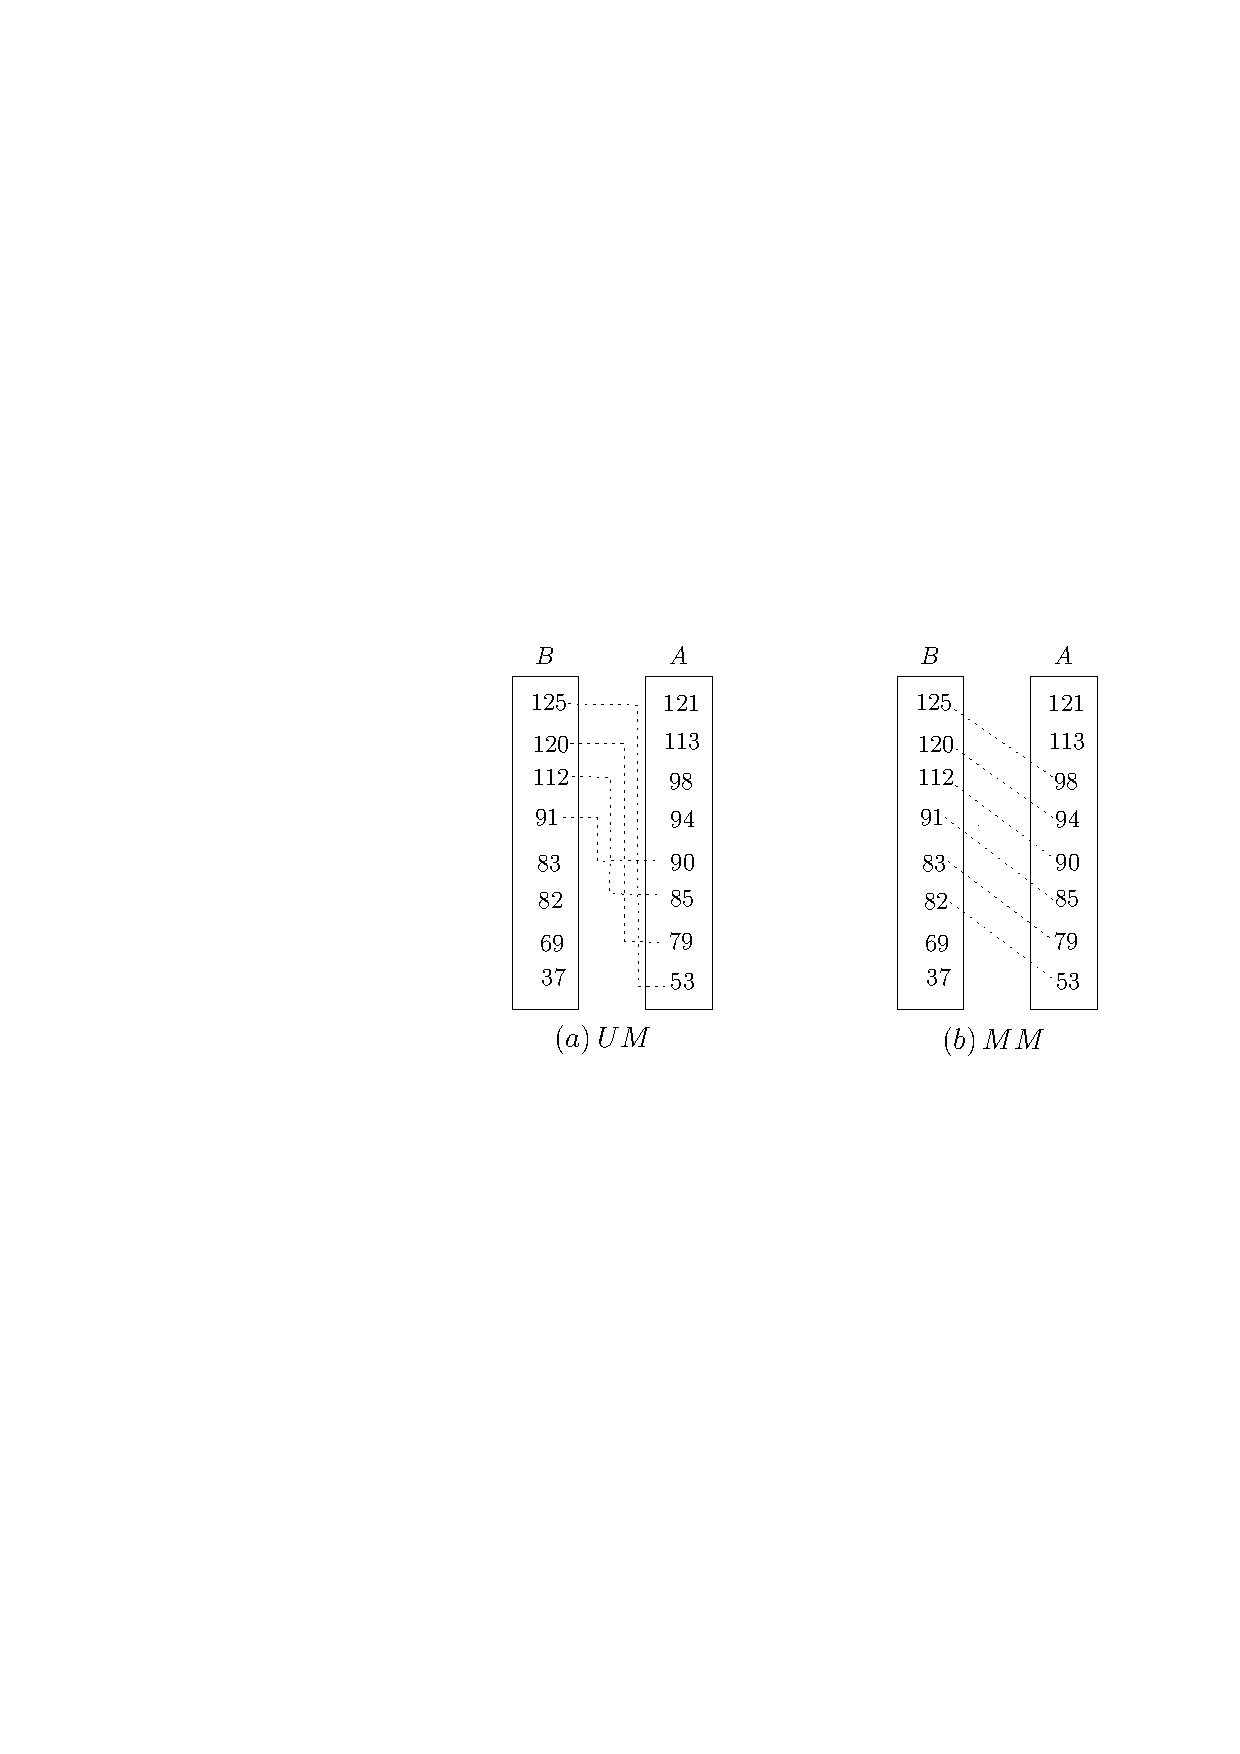
\includegraphics[width=0.5\textwidth]{UM.pdf}
\caption{(a) The dotted lines indicate all the bid-ask pair  produced by function \tw{produce\_UM}. In each iteration function \tw{produce\_UM}  matches the largest available bid in $B$ with the smallest available ask in $A$.  (b) The dotted lines here indicate a maximum matching for the list of bids $B$ and list of asks $A$. Note that in this case the matching produced by \tw{UM} is not a maximum matching. }
\label{fig:UM}
\end{figure}

\textbf{Proof}: Let $M$ be any arbitrary IR and uniform matching on the list of bids $B$ and list of asks $A$ where each matched bid-ask pair is traded at price $t$. We need to prove that $m \leq$ |\tw{(UM $B$ $A$)}| where $m$ is the number of matched bid-ask pairs in the matching $M$. Observe that in any individually rational and uniform matching the number of bids above  the trade price is same as the number of asks below the trade price (See Fig~\ref{fig:UM_match}). Therefore, there are at least $m$ bids above $t$ and $m$ asks below $t$ in $B$ and $A$ respectively. 

\begin{figure}[h!]
\centering
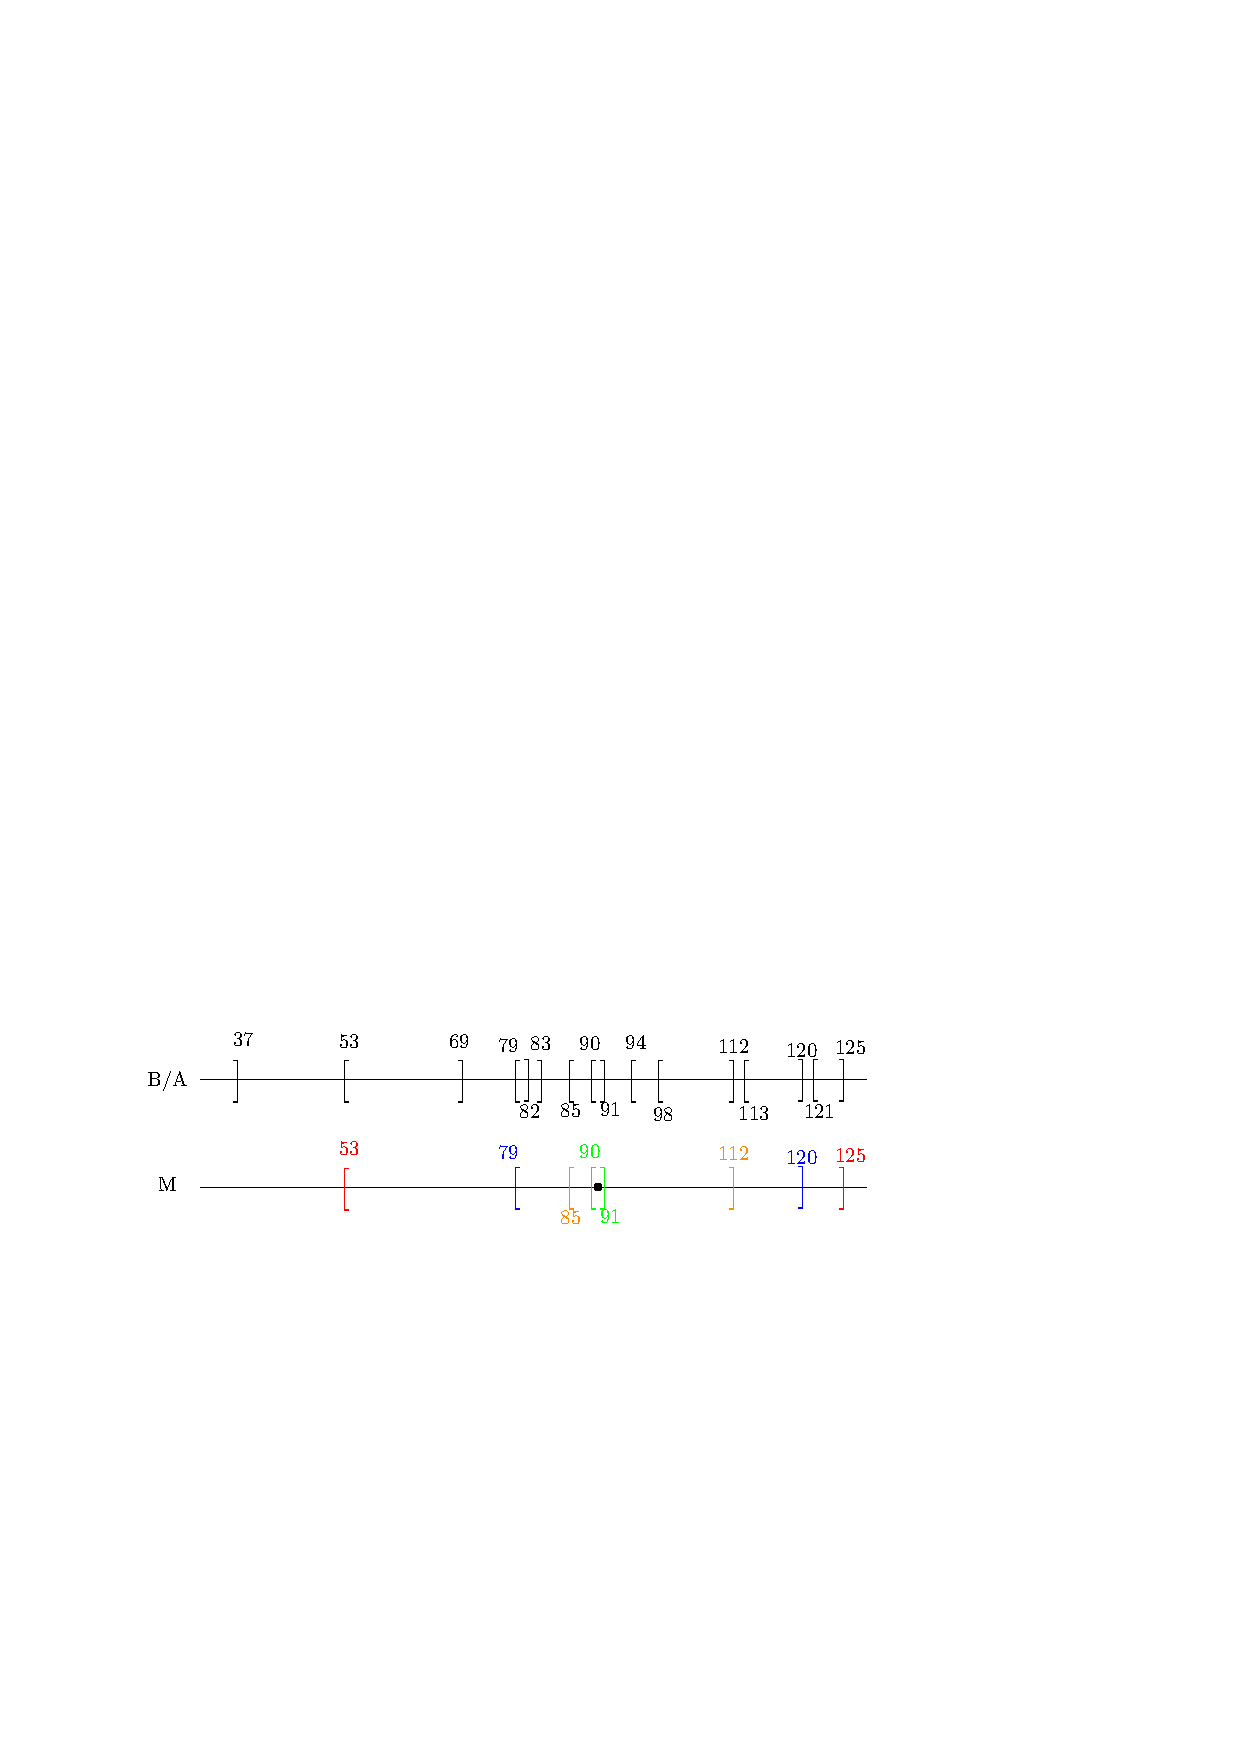
\includegraphics[width=0.8\textwidth]{UM_matching.pdf}
\caption{ Trade price $p$ for the matching $M$ is shown using a dot that lies between the ask with limit price 90 and bid with limit price 91. Note that since $M$ is individually rational the number of matched asks below the trade price $p$ is same as number of matched bids above the trade price $p$. }
\label{fig:UM_match}
\end{figure}

Since at each step the function \tw{produce\_UM}  pairs the largest bid available in $B$ with the smallest ask available in $A$ it must produce  at least $m$ bid-ask pairs. Hence for the list of bids $B$ and list of asks $A$ the function \tw{UM} produces a uniform matching which is of size at least $m$. $\square$


\subsection{Double sided auction in financial markets}
TODO

\section{Conclusion}\label{sec:conclusion}
There are several algorithms known for double sided auctions \cite{Deshmukh:2002:TCD}. For many applications of double sided auctions, fairness, individual rationality and uniformity are some of the essential properties required. Theorem provers can be a useful tool in the analysis of these properties. Formalizing an algorithm for double sided auctions in a theorem prover increases its reliability. Previously there has been works that formalizes some of the concepts from microeconomics \cite{toolbox,welfare} in a theorem prover. There is also an  attempt by Passmore et al. to formalize financial markets \cite{PassmoreI17}. Our work, to the best of our knowledge, is the first attempt to formalize double sided auction mechanisms in a theorem prover.

We formally define various notions of double sided auctions in the Coq Proof Assistant.
Moreover, we prove some general results on matchings in a double sided auction. We use
lists to define the notion of a matching. To express the properties
of various processes operating on a matching we define some relations on lists. We develop a library of facts on these relations which is further used to prove
important results on matchings in a double sided auction. Finally, we use this formal setting
to verify properties of two important classes of matching algorithms known as dynamic price
and uniform price algorithms. In this work, we assume that each trader wishes
to trade a single unit of product and the product is indivisible. In the future this work can be
extended to accommodate trades involving multiple units of an item. Another interesting direction of work
would be extending this framework to include the analysis of continuous markets as well.

%% Bibliography
\bibliography{auction}

\end{document}
